\chapter{INTRODUÇÃO}

\section{JUSTIFICATIVA}

Sabe-se que o campo de trabalho para os novos dos profissionais atuantes na área das ciências agrárias tem mudado, a busca pela valorização das capacidades e competências profissionais. Busca-se cada vez mais a afirmação e promoção de direitos de cidadania, associatividade política, responsabilidade social e ambiental, consideração, respeito as diversidades étnicas e culturais que devem ser valorizadas constantemente, para tal, a academia  tem um papel importante neste contexto, que é  o de fomentar e oportunizar essas competências. Dentro deste contexto a capacidade de manter-se fio a inovação, especialmente a destrutiva é fundamental ao progresso do crescimento e manutenção futura do profissional das agrárias no novo mercado de trabalho, assim como saber lidar com os novos empreendimentos nos campos de atuação.


De acordo com \citeonline{tarapanoff_monitoramento_2016}, existe um cenário favorável para os negócios rurais que buscam a sustentabilidade econômica e ambiental. Nesse sentido o Brasil deve buscar trilhar  um caminho seguro em relação à sustentabilidade de seu agronegócio, em consonância com as melhores práticas da exploração ambiental e a produção agrícola, parte promovida por cumprimentos a regras ambientais a exemplo a Agenda 2030 que prevê a exploração consciente dos recursos naturais e tomando medidas urgentes sobre a mudança climática individuais quanto institucionais, \cite{filho_documentos_2017}.


O desenvolvimento sustentável pode ser definido segundo \cite{lara_ideologia_2017} como um negócio socialmente responsável e ecologicamente correto, mas invariavelmente viável em termos financeiros. Concomitantemente existe uma lacuna na formação profissional durante o ensino superior no que se refere à adoção de uma cultura empreendedora, \cite{lima_ser_2015}. Não tem sido possibilitado aos acadêmicos, a oportunidade de gerar inovação tecnológica sustentável, inclusive como forma de aplicação prática dos conhecimentos adquiridos. Da mesma maneira, é sabido que para uma ideia inovadora alcançar o sucesso desejado é preciso muito mais que o conhecimento técnico. É necessário que seja disponibilizado aos futuros profissionais/empreendedores treinamento na formulação das ideias em etapas direcionadas e adequadamente orientadas.


Para que um negócio sustentável possa ter sucesso é preciso mais do que uma ideia inovadora, deve ter o meio e os profissionais capacitados para tal, Relatórios da Fundação Kauffman afirma que as Startups criam uma média de 3 milhões de novas vagas de empregos anualmente e que, estes tipos de empreendimentos serão responsáveis pela criação de mais de 50\% dos empregos no  mundo  \cite{brasil_o_2017}. Atualmente estes tipos de  negócios contribuem para o crescimento de diversas regiões geográficas, já que não se expandem apenas em tamanho, mas também em novos locais, além de incentivar o emprego em suas indústrias relacionadas. Supletivamente, como muitas dessas microempresas são responsáveis por desenvolver novas tecnologias e processos, elas também geram aumento de absorção do capital humano mais capacitado para gestão e gerência.


Diante deste cenário, para que o aprendizado dos profissionais seja mais efetivo, surgem diversas abordagens e metodologias a serem assimiladas. Nesse contexto, deve existir uma maior produção de estudos e conteúdos sobre a educação empreendedora e os modelos educacionais que melhor se apliquem ao aprendizado deste, como ressalta \citeonline{kuratako_entrepreneurship_2003}. É notória a urgência de se pesquisar o ensino em empreendedorismo de forma disciplinada no meio acadêmico. Por ser um tema de grande importância, a educação empreendedora promovida no seio da educação superior pode ser o caminho para o surgimento de inovações sustentáveis e economicamente viáveis passives e escaláveis.


Dentro do contexto metodológico educacional, temos as metodologias ativas, que trazem a possibilidade de mudança da centralidade no docente (ensino) para o estudante (aprendizagem), ponto de vista preconizado por \citeonline{freire_pedagogia_1987} ao abordar educação como um processo que não é realizado por outrem, ou pelo próprio indivíduo, mas que acontece na interação entre pessoas através de sua vivência por meio de palavras, ações e reflexões. Enquanto o método tradicional de ensino utiliza a transmissão de informações e concentra as atividades no docente, no método ativo, os alunos ocupam a centralidade da educação e o conhecimento é construído de forma colaborativa. Sucintamente, as metodologias ativas propõem transformar o processo de ensino e aprendizagem na busca pelo comportamento empreendedor, como uma forma de enfrentar o modelo tradicional praticado e aceito ao longo dos anos.
 

As práticas ativas estimulam o reconhecimento dos problemas do mundo atual, tornando os alunos aptos a intervir na promoção das transformações necessárias a exemplo as que se baseiam  na reflexão e argumentação \cite{bezanilla_methodologies_2019}. Assim, o aluno torna-se protagonista da sua aprendizagem e autônomo no alcance dos seus objetivos incorporando seus valores e razões \cite{rubel_student_2016}. Existem vários recursos, ferramentas e estratégias para alcançar o satisfatório comportamento empreendedor, como: uso de tecnologias digitais e aplicativos \cite{pereira_use_2020}, ensino híbrido e suas estratégias como sala de aula em rotação por estações, Aprendizagem Baseada em Problemas (ABP) \cite{souza_aprendizagem_2015}, e uso de situações-problema e estudos de caso, sala de aula invertida \cite{junior_sala_2016,branco_sala_2016}, uso de mapas mentais \cite{junior_percepcao_2018}, sala de aula compartilhada \cite{strack_por_2009}, estratégias de Design Thinking \cite{andrews_circular_2015}, Gamificação \cite{ogawa_avaliacao_2016}, projetos de extensão \cite{garcia_contribuicao_2012}, dentre tantos outros recursos do método ativo, os quais podem vir facilitar o entendimento e a compressão dos acadêmicos das Ciências Agrárias no contexto de um mercado de trabalho que se apresenta com um perfil voltado ao empreendedor.

O empreendedorismo é a capacidade de reunir esforços para transformar em realidade uma oportunidade, objetivando a satisfação pessoal do empreendedor e o lucro. Tal conceito define o empreendedorismo como uma prática constante das atividades rotineiras dos educandos. Desde a capacidade de resolução de problemas quanto a idealização de propostas capazes de inovar. Dentro desta dicotomia entre empreendedorismo e educação surge a "Educação Empreendedora", que por meio de práticas e dinâmicas planejadas busca a melhora na promoção do comportamento empreendedor \cite{martins_educacao_2016, morais_empreendedorismo_2018}, e resolução de problemas de forma sustentável e rápida.

É diante desta problemática que este projeto busca avaliar a inovação sustentável e a eficácia da promoção empreendedora por meio de uma ação de educação com vistas aos negócios rurais, por meio do Programa Empreenda Agro Sustentável promovido para os acadêmicos das ciências agrárias, utilizando para este fim, Workshops encadeados e ferramentas didáticas que buscam capacita-los para a construção de propostas inovadoras viáveis.


\section{DELIMITAÇÕES DO ESTUDO}

Esta pesquisa está focada na dissonância entre a teoria e pratica dos métodos educacionais e as mudanças vertiginosas do mercado de trabalho no meio rural. Este Setor foi escolhido por estar contribuindo significativamente para a balança comercial do país, apresentando saldos positivos frequentes. Da mesma forma contribui para a segurança alimentar do País e produção de produtos limpos e renováveis. O mercado emergente apresenta significativa contribuição para a empregabilidade da população no campo, invertendo cada vez mais o êxodo rural, porém este mercado que absorve novos profissionais, exige que tais profissionais se mostrem a cada dia mais capacitados para lidar com o desenvolvimento tecnológico e a produção em larga escala, em que a busca pela valorização das capacidades e competências profissionais aumenta a cada dia. 

Em contraponto o empreendedorismo atualmente se confunde com a Meritocracia. Tantos a meritocracia quanto o empreendedorismo caminham junto no cerne do movimento de individualização no mundo do trabalho \cite{noauthor_empreendedorismo_nodate}. Os dois  Projetam imagens individuais de trabalho e sucesso, em que a capacidade individual somada as oportunidades geram resultados positivos junto ao mercado de trabalho. Porém a diferença substancialmente positivos. Porém o Empreendedorismo derivado da educação empreendedora proposto neste projeto, surge atrelado a técnicas e métodos capazes de facilitar e validar as propostas empreendedoras, assim sendo um programa que vise o incentivo as práticas empreendedoras de forma sistemática e coerentes distingue dos resultados negativos que estão atrelados a meritocracia e suas vantagens a frente dos pares distintos.

Visando compreender o comportamento empreendedor nos alunos dos cursos do Centro Ciências Agrárias Aplicadas CCAA da Universidade Federal de Sergipe-UFS, foi escolhida a população para esta pesquisa de 1.453 discentes dos cursos de graduação nas áreas de agrárias da Universidade Federal de Sergipe (UFS): Engenharia Agronômica, Engenharia Agrícola, Zootecnia, Engenharia Florestal, Veterinária e Engenharia de Pesca, dados contidos no relatório estatístico de matriculas 2017 da instituição. A amostra compreenderá  120 discentes que participarem do programa Empreenda Agro Sustentável.

As atividades serão desenvolvidas por meio de quatro Workshops, que constam metodologias ativas, oficinas, palestras com vistas a promover aprendizagem significativa e colaborativa. Durante os módulos do projeto (Workshops), os participantes testarão de seus \textit{insights} para que novas requisições sejam realizadas e/ou que erros nos planejamentos sejam encontrados e, consequentemente, debatidos e mitigados. Depois que todas as Sprints (atividades dos três Workshops) forem finalizadas, ou seja, que todos os módulos sejam abordados, será iniciado um ciclo de Apresentações e desenvolvimento da habilidade de apresentação e demonstração dos produtos por meio apresentações (Pitch). O programa será desenvolvido em quatro encontros (Workshops), que abordarão temas pertencentes ao empreendedorismo e o comportamento empreendedor, a saber: 

\begin{itemize}

\item {1º Workshop: O que é Startups, Empreendedorismo, comportamento empreendedor e cultura empreendedora, Problemas (segmentação do mercado), segundo os Objetivos do Desenvolvimento Sustentável (ODS), Modelagem do negócio e Criatividade;}
\item {2º Workshop: A busca de oportunidades como Característica Empreendedora, Construção do Lean Canvas, Mapa de Empatia, Validação da Proposta de Valor e Economia colaborativa e Coworking; }

\item {3º Workshop: Makeathon: Prototipagem para o MVP, O que você pode fazer por seu cliente e como o cliente adquire seu produto?;}
\item {4º Workshop: Demoday. Destaca-se que o instrumento de pesquisa que será utilizado neste experimento foi composto por Cinco blocos de questões de múltipla escolha baseadas principalmente em escalas de cinco ou sete possibilidades.}
\end{itemize}

O  primeiro conjunto de questões está relacionado a informações que buscam traçar o perfil dos alunos entrevistados, tais como: gênero, faixa etária, curso vinculado e o perfil de interesse nas áreas de estudo ligadas ao empreendedorismo sustentável tal questionário foi baseado no trabalho desenvolvido por \citeonline{lima_ser_2015}. O segundo bloco e composto por 10 questões relacionadas a auto eficácia dos estudantes de múltipla escolha partindo da alternativa “Completamente Inseguro” a "Completamente Seguro”. O terceiro bloco e composto por 7 questões que analisam a intenção empreendedora do aluno da quais segue uma proporção partindo da resposta, tendo como alternativas partido do “Discordo totalmente” a “Concordo totalmente”. O Quarto bloco retrata a intensão ter sua própria empresa ou ser autônomo e por fim o Quinto bloco contendo 11 questões sobre a ligação da família e o apoio familiar no empreendedorismo, tendo como alternativas partido do “Discordo totalmente” a “Concordo totalmente”. Buscando aferir os resultados do programa, um novo questionário abordando as mesmas temáticas será aplicado ao final do programa. 
O estudo caracteriza-se como uma pesquisa de levantamento ou Survey, que se destaca por compreender uma amostra expressiva em relação ao universo pesquisado. Optou-se por adotar a abordagem qualitativa para a análise dos dados quanto a percepção do comportamento empreendedor dos alunos, e a abordagem quantitativa na mensuração dos resultados educacionais do Programa Empreenda Agro Sustentável. Após a aplicação dos instrumentos de análise, será realizada a categorização dos dados para que seja possível a classificação da pontuação segundo o questionário GUESS que utilizada testes de hipóteses sobre uma proporção. O projeto traz como benefícios: 

\begin{itemize}
\item{Promover o desenvolvimento pessoal, econômico e social no meio rural por meio de oportunidade de acesso a alternativas de geração de renda;}
\item{Criar a oportunidade de se trabalhar com o que realmente gosta e vencer os entraves do mercado econômico;}
\item{Dar autonomia e liberdade para conduzir o próprio talento, porem orientado por metodologias especificas;}
\item{Transmitir valores e inspirar novos empreendedores no ambiente agrário;}
\item{Ensinar como lidar com os fracassos e frustrações, sabendo como contorna-los;}
\item{Ensinar estratégias de planejamento de ideias ou carreiras buscando geração de renda;}
\end{itemize}


\section{OBJETIVOS}

\subsection{OBJETIVO}

Avaliar o impacto do Programa Empreenda Agro Sustentável como mecanismo indutor de competência empreendedora com inovação no setor do agronegócio junto aos acadêmicos das Ciências Agrárias da UFS.



\subsection{OBJETIVOS ESPECÍFICOS}

\begin{itemize}
\item{Identificar o efeito da promoção de iniciação empreendedora direcionado a inovação sustentável no meio acadêmico;}
\item {Avaliar o potencial empreendedor dos alunos do Centro de Ciências Agrárias Aplicadas participantes do Programa;
}
\item {Fomentar por meio do projeto de extensão o comportamento empreendedor nos alunos do Centro de Ciências Agrárias Aplicadas;}

\item {Tipificar e analisar os tipos de PI que surgem com o incentivo ao empreendedorismo sustentável por meio da aplicação das metodologias trabalhadas no Programa.}

\end{itemize}


\section{PROBLEMA}

O comportamento empreendedor como indutor de inovação, pode ser estimulado mediante o uso de projetos de extensão universitária como o Programa Empreenda Agro Sustentável? 


\section{HIPÓTESE}

Programas que trabalham a promoção do comportamento empreendedor no meio acadêmico promovem o surgimento de inovação.

%\section{RISCOS}
%\begin{itemize}
%\item{Tomar parte do tempo do entrevistado ao responder ao questionário/entrevista;}
%\item{Risco a segurança dos prontuários;}
%\item{Considerar riscos relacionados à divulgação de imagem, quando houver filmagens ou registros fotográficos;}
%\item{Cansaço ou dispersão ao responder questionários;}
%\end{itemize}





%%%%%%%%%%%%%%%%%%%%%%%%%%%%%%%%%%%%%%%%%%%%%%%%%%%%%%%%%%%%%%%%%%%%%%%%%%%%%%%%%%%%%%%%%%%%%%%%%%%%%%%%%%%%%%%%%%%%%%%%%%%%%%%%%%%%%%%%%%%%%%%%%%%%%%
                                                                 %REFERENCIAL TEÓRICO%                                                                             
%%%%%%%%%%%%%%%%%%%%%%%%%%%%%%%%%%%%%%%%%%%%%%%%%%%%%%%%%%%%%%%%%%%%%%%%%%%%%%%%%%%%%%%%%%%%%%%%%%%%%%%%%%%%%%%%%%%%%%%%%%%%%%%%%%%%%%%%%%%%%%%%%%%%%%
%%%%%%%%%%%%%%%%%%%%%%%%%%%%%%%%%%%%%%%%%%%%%%%%%%%%%%%%%%%%%%%%%%%%%%%%%%%%%%%%%%%%%%%%%%%%%%%%%%%%%%%%%%%%%%%%%%%%%%%%%%%%%%%%%%%%%%%%%%%%%%%%%%%%%%


\chapter{REFERENCIAL TEÓRICO}

\section{Desenvolvimento Rural Sustentável}

Definir o desenvolvimento do meio rural requer um considerável esforço observacional e prático, pois este ambiente vem sofrendo profundas transformações em suas demandas e necessidades, o que antes apresentava essencialmente produção de subsistência, hoje da lugar a um complexo sistema agroindustrial \cite{bastos_determinantes_2018}. Importante neste sentindo compreender que definir o desenvolvimento rural com apenas um conceito seria uma proposição simplista do contexto desenvolvimento rural.

Partindo da definição de consequência de ações governamentais definidas por \citeonline{navarro_desenvolvimento_2001} como "ações práticas" este autor descreve que o:


\begin{citacao}
“[...] Desenvolvimento rural, portanto, pode ser analisado a posteriori, neste caso referindo-se às análises sobre programas já realizados pelo Estado (em seus diferentes níveis) visando a alterar facetas do mundo rural a partir de objetivos previamente definidos. Mas pode se referir também à elaboração de uma "ação prática".
\end{citacao}


O desenvolvimento também pode ser compreendido por meio de um conceito mais regional definido como "desenvolvimento local". Tal expressão é recente e deriva de iniciativas de mobilização organização social no sentido de promover uma maior representação dos diferentes atores sociais no processo de desenvolvimento. E que o Estado assume papel de agente facilitador desse processo de descentralização das políticas públicas  para ser democrático, a transparência de suas instituições, o equilíbrio das forças exercidas pelas diferentes correntes de interesse e o compromisso com a qualidade de vida na população afetada \cite{campanhola_diretrizes_2000}. Tal conceito ver o espaço rural como um local ideal para a promoção de políticas de inovação e a construção de padrões inovadores na relação entre populações e instâncias públicas, numa tentativa de rompimento com a dominação, que parte de baixo para cima. Neste contexto surge as Organizações Não Governamentais ONGs que buscam garantir a participação da população local, e fazer valer tais mudanças atuando normalmente em ambientes geograficamente mais restritos (a região rual, povoados ou o municípios), \cite{assis_agricultura_2005, campanhola_diretrizes_2000}.


E por fim, a aqui pretendida a ser direcionada com estes estudos: "desenvolvimento rural sustentável". O Conceito que surge derivado do termo "Progresso", antes entendido genericamente como sentido parcial e prático de “melhoramento do ambiente” \cite{almeida_da_1995}. Entretanto, torna-se imprescindível destacar que, o desenvolvimento sustentável no meio rural não pode ter suas bases de compreensão apenas no desenvolvimento econômico, local ou regional. Se mostra de suma importância entender que compreender o desenvolvimento de forma sustentável é necessário ter um olhar sistêmico que permeie todo o processo, envolvendo diversas dimensões, dentre as quais se destacam a econômica, a sociocultural, a político-institucional e a ambiental \cite{vieira_politica_2015}, a ação de desenvolvimento sustentável é por um lado fruto do desenvolvimento social, por outro lado esta ação contribui com o desenvolvimento da sociedade de forma autossustentável, ao introduzir inovações sem ser predatória, ao satisfazer demandas específicas tendo como base a economia circular e ao tornar mais densas as redes de cooperação buscando a autossuficiência consciente  satisfazendo as necessidades no presentes, sem comprometer a capacidade das gerações futuras de suprir suas próprias necessidade \cite{onu_sustainable_2016}.

No Brasil o desenvolvimento rural propriamente dito teve início com a politica de “intensificação verde”, por meio da revolução verde, plano politico que teve força de ação iniciando nos anos 60 e 70. Tal política era baseada em subsídios de créditos que buscava o estimulo a produção agrícola em larga escala principalmente de \textit{commodities}, da mesma forma impulsionada por diversas políticas direcionadas a estimular o crescimento do setor, entre elas a política de expansão da malha rodoviária, políticas específicas de crédito rural, preços mínimos, pesquisa e extensão rural \cite{kageyama_o_1990}. Os incentivos e créditos que de fato chegaram ao campo, foram em sua maioria utilizadas por empresas de maquinários e de insumos industriais para uso agrícola \cite{strassburg_producao_2015}, incentivado apenas o aumento da produção em escala industrial, deixando de lado as preocupações com a manutenção dos recursos limitados no campo e a capacidade de escalabilidade dos pequenos produtores.

Tal desenvolvimento teve como ponto positivo o estreitamento das fronteiras entre o meio rural e o meio urbano, tornando-as cada vez mais tênues e difusas \cite{freitas_mudancas_2012}, já que a sociedade civil emerge como protagonista desse processo de construção dos pilares para um desenvolvimento mais responsável e abrangente \cite{de_souza_empreendedorismo_2016}. 

Desta forma a produção agrícola atual além do dever de entregar as necessidades alimentares da população, hoje requer acompanhar ainda mais as necessidades da população como um tudo urbana, tais como: Produtos com maior qualidade, rapidez e efetividade na entrega, volume cada vez maior, entre outros. hoje o pensar em tecnologias inovadoras para o campo, requer uma essencial compreensão entre as necessidades do meio urbano e as possíveis capacidades do meio rural e que este mantenha-se auto-sustentável em todas as dimensões ambientais, sociais e culturais, sendo de suma importância a compreensão do que de fato venha ser o rural e como construir sua sustentabilidade, as soluções propostas para superar esses desafios devem não apenas considerar a maneira como os alimentos são produzidos, mas também cuidar de preocupações sociais, ambientais e econômicas \cite{noauthor_achieving_2020}. 

O rural deve ser visto segundo \cite{kageyama_desenvolvimento_2008} como um amálgama de práticas heterogêneas, estilos mutuamente contrastantes, tendências de desenvolvimento divergentes, posições hegemônicas e mudanças quase subterrâneas que, a princípio, são praticamente imperceptíveis, mas que, por fim, podem mudar a todo o sistema de produção. Compreender a complexidade do rural se faz necessário avista que a simples padronização do ambiente, deixando de lado o conceito reducionista que o campo é uma concisa do que ocorre no rural \cite{van_der_ploeg_trajetorias_2011}. 

Umas das ferramentas possíveis para promoção de um desenvolvimento que leve em consideração as complexidades do campo é o empreendedorismo e o uso por meio da efetiva e direcionada aplicação, porem se faz necessário compreender melhor o que vem a ser o empreendedorismo e as aplicações de forma sustentáveis como também suas ligações com ao campo se faz necessário compreender os conceitos de empreendedorismo e sustentabilidade, como também a aplicação prática no meio rural. 

Segundo \citeonline{dornelas_como_2003}, o empreendedorismo significa fazer algo novo, diferente, mudar a situação atual e buscar, de forma incessante, novas oportunidades de negócio, tendo como foco a inovação e a criação de valor. Diversas são as definições de empreendedorismo e o empreender, mas a essência resume-se no inovar, criar algo novo ou modificar algo buscando uma nova aplicação e fazer diferente, empregar os recursos disponíveis de forma criativa, assumir riscos calculados, buscar oportunidades e inovar, podendo ser o processo de criação de valor tendo em vista limitados recursos e capacidade de aplicação tornando capitalizável e economicamente viável \cite{costa_empreendedorismo_2006, stevenson_new_1989, lopes_educacao_2010}. Apesar dessa diversidade conceitual, a ideia de empreendedorismo tem sido predominantemente associada às concepções de progresso e tecnológico usual deixando de lado o campo e nele suas aplicações praticas.  

O intenso debate sobre desenvolvimento da agricultura brasileira de forma sustentável em consonância com assuntos econômicos de interesse nacional torna o tema deste trabalho oportuno e atual, haja vista que a agricultura no Brasil responderam por 19\% do total das exportações no ano de 2018, \cite{mdic_comex_2019}, porém este meio de produção convive com a  limitação dos recursos naturais \cite{jacobi_meio_1999}, levando ao estado pensar em políticas públicas que busquem soluções para as demandas tecnológicas surgidas no meio rural, e gerar profissionais capazes compreender a complexidade da intensa produção no campo mantendo o ritmo constante das mudanças tecnológicas ao mesmo tempo o uso de limitados recursos naturais  \cite{costa_dinamica_2016}, um profissional empreendedor.
No alcance desse modelo sustentável, tal profissional deve ser preparado desde a academia por meio da educação empreendedora a lidar e estar capaz de melhorar o desempenho produtivo \cite{da_silva_qualidade_2017}, a capacidade competitiva a melhoria da segurança alimentar do pais \cite{hoffmann_brasil_2014}, e ao mesmo tempo garantir a perpetuação da manutenção do meio ambiente, e não apenas replicar novos padrões de produção e distribuição de bens e serviços e do uso dos recursos naturais, ele devem ser capazes de inovar \cite{morais_empreendedorismo_2018}.

Sobre tais bases, conclui-se que o desenvolvimento do campo de forma tradicional disporia de poucas chances além da alternativa de uma prática intensiva em capital e exploração dos recursos naturais, cuja intensificação e amplitude pode levar a escarces dos meios \cite{costa_agrarian_2016}. 



\section{Comportamento Empreendedor e Educação empreendedora}


O Investimento no  capital  humano desde a formação permite  melhorias  no fator trabalho e aumenta os níveis de produtividade e renda dos profissionais \cite{macedo_capital_2019}. Até pouco tempo, os currículos educacionais nas escolas e cursos relacionados a administração no Brasil focavam quase que totalmente ao atendimento às necessidades do mundo corporativo, deixando de lado o fator criatividade e inovação buscando resolução de risco de seus alunos em vez de formar líderes criativos que assumam riscos \cite{sanna_evolution_1999}. O mercado emergente, a necessidade de entrega urgente, a redução das ofertas de emprego levaram os centros de ensino a iniciar o desenvolvimento desta disciplina e os conteúdos relacionados. É nesse contexto que surge o ensino do empreendedorismo no Brasil tendo como precursor o Professor Ronald Degen \cite{koerner_designing_1990} na Escola de Administração de Empresas de São Paulo (EAESP) da Fundação Getúlio Vargas (FGV), em 1981. Contudo, é vasta a literatura voltada para o tema e podemos destacar os trabalhos de  \citeonline{dolabela_oficina_1999}; \citeonline{duarte_sesi_2004}; \citeonline{pires_empreendedorismo_2006}; \citeonline{ramos_o_2005}, \citeonline{branca_terra_o_2006} entre outros. O Quadro \ref{tabela_1} desenvolve um recorte histórico do ensino da área no Brasil, tendo como corte temporal 1980 a 2007, segundo \cite{fernandes_breve_2013}. 


%Quadro1%%

\begin{table}[htb]
\caption{\label{tabela_1}\textbf{Histórico do Ensino de Empreendedorismo no Brasil}}
\begin{tabular}{p{1.5cm}p{13.0cm}}
\hline \hline
1980 & Fundação Getúlio Vargas - FGV implanta o ensino formal de empreendedorismo no Brasil;  \\\hline
1980 & A Universidade de São Paulo - USP institui polo de ensino de empreendedorismo;  \\\hline
1981 & O Professor Ronald Degen leciona a disciplina “Criação de Negócios”  \\ \hline
1984 & O Professor Sílvio dos Santos, da USP leciona disciplina referente à criação de novas \\ \hline
1989 & O Professor Degen publica o livro “O empreendedor: fundamentos da iniciativa empresarial”;  \\\hline
1991 & A Professora Ofélia Sette Torres funda o Centro de Empreendedorismo;  \\\hline
1991 & É introduzido no Brasil o Programa Empretec, da Organização das Nações Unidas - ONU, para
capacitar empreendedores;  \\\hline
1993 & O Empretec passa a ser coordenado pelo Sebrae no Brasil;  \\\hline
1996 & O Professor Paulo Goldsmith, coordena a versão brasileira da competição internacional Global Moot Corp, realizada pela Universidade do Texas desde 1984. Em 2001 essa competição foi aberta a todas as escolas da América Latina, passando a se chamar Latin America Moot Corp;\\\hline
1999 & Lançamento do livro “O Segredo de Luísa”, do Professor Fernando Dolabela, renomado
especialista em educação empreendedora no Brasil e criador da Pedagogia Empreendedora;  \\ \hline
2000 & Os professores Tales Andreassi e Marcelo Aidar passam a ministrar curso de empreendedorismo
na EAESP;  \\ \hline
 2002 & O Professor José Antônio Lerosa de Siqueira funda na USP o Centro Minerva de Empreendedorismo;  \\\hline 
   2005 & É realizada a primeira Semana do Empreendedorismo pelo Centro de Empreendedorismo e Novos Negócios da FGV. Atualmente o centro é o responsável pela Latin America Moot Corp e pela competição Sumaq16 de empreendedorismo social;  \\\hline 
   2007 & A FGV é pioneira ao estabelecer como obrigatórias disciplinas que tratem do tema empreendedorismo nas grades curriculares dos cursos de graduação em administração pública e de empresas da EAESP; \\\hline 
\end{tabular}
 \fonte{\raggedright\cite{almeida_aprendizagem_2019}}
\end{table}

\clearpage
Fica nítido que a preocupação com o ensino de empreendedorismo está saindo de sua fase embrionária e se consolidando nos principais centros de graduação e pós-graduação, nos mais diversos segmentos de formação desde cursos de engenharia, passando por desenho industrial, até o turismo \cite{henrique_praticas_2008}. A educação empreendedora como forma de investimento ao capital humano a além de fortalecer o fornecimento de novos produtos e a dinamização de atividades  econômicas, torna-se uma possibilidade para se combater o desemprego \cite{morais_empreendedorismo_2018} e o aumento das jornadas de trabalho. Para \citeonline{schaefer_formacao_2017}, o indivíduo empreendedor é o ator capaz de inovar no processo evolutivo do mundo contemporâneo, capaz de resolver problemas e absorver oportunidades, atribuindo-se este sujeito como agente de mudança e capaz de lidar com as contantes inversões do mercado de trabalho. 

Com as Universidade e Institutos de ensino superior sendo reconhecidamente contextualizados como promotores da inovação no  Brasil, pais que configura o 13º lugar entre os maiores produtores de publicações de pesquisa (\textit{papers}) e inovação a nível mundial, \citeonline{clarivate_analytics_web_of_research_2017}.  O novo paradigma educacional, portanto, situa as instituições de ensino superior no campo da promoção do empreendedorismo direcional e sistemático, assim como o comportamento empreendedor, visto que, a educação empreendedora disciplinada mostra-se eficaz no tocante ao surgimento da inovações melhor direcionadas e a promoção da identidade empreendedora para novos negócios, \cite{jain_academics_2009} já que a universidade vem a ser um local privilegiado do saber, da liberdade acadêmica e da inteligência, em que o conviver com a pesquisa na fronteira do tem a capacidade de propagação tendo o poder de ‘oficializar’ o empreendedorismo como um conteúdo de conhecimento” \cite{dolabela_oficina_2008}. Uma vez que a formação empreendedora envolve uma série de conteúdos de aprendizagem, faz-se necessário organizar as diversas metodologias com as respectivas aplicações pedagógicas, \cite{rocha_avaliacao_2014} elencou os Principais Métodos, Técnicas e Recursos Pedagógicos no Ensino de Empreendedorismo. 



\begin{center}

\begin{longtable}{p{3.5cm}p{11.0cm}}

\caption[\textbf{Principais Métodos, Técnicas e Recursos Pedagógicos no Ensino de Empreendedorismo}]{\textbf{Principais Métodos, Técnicas e Recursos Pedagógicos no Ensino de Empreendedorismo}} \label{tabela_2} \\


\hline \multicolumn{1}{p{3.5cm}}{\textbf{Métodos, Técnicas e Recursos}} & \multicolumn{1}{c}{\textbf{Aplicações}}\\ \hline 

\endfirsthead


\multicolumn{2}{c}%

{{\bfseries \tablename\ \thetable{} — Continuação}} \\

\hline \multicolumn{1}{p{3.5cm}}{\textbf{Métodos, Técnicas e Recursos}} & \multicolumn{1}{c}{\textbf{Aplicações}}  \\ \hline 

\endhead

\hline \multicolumn{2}{r}{{Continua}} \\ \hline

\endfoot


\hline \hline

\endlastfoot

Aulas expositivas & Transferir conhecimentos sobre o Empreendedorismo, as características pessoais do empreendedor, os processos de inovação, fontes de recursos, financiamentos e aspectos legais de pequenas empresas.  \\

Visitas e contatos com empresas & Estimular o \textit{network} e incitar o estudante a sair dos limites da IES para entender o funcionamento de mercado na vida real. Desenvolver visão de mercado.  \\

Plano de negócios & Desenvolver as habilidades de planejamento, estratégia, marketing, contabilidade, recursos humanos, comercialização. Desenvolver a habilidade de avaliação do novo negócio, analisando o impacto da inovação
no novo produto ou serviço. Construir habilidade de avaliar e dimensionar riscos do negócio pretendido. \\ 

Estudos de casos & Construção da habilidade de pensamento crítico e de avaliação de cenários e
negócios. Desenvolver a habilidade de interpretação e definição de contextos associados ao Empreendedorismo. \\ 

Trabalhos teóricos em grupo & Construção da habilidade de aprender coletivamente. Desenvolver a
habilidade de pesquisar, dialogar, integrar e construir conhecimentos,
buscar soluções e emitir juízos de valor na realização do documento escrito. \\ 

Trabalhos práticos em grupo & Construção da habilidade de atuar em equipe. Desenvolver a habilidade de
planejar, dividir e executar tarefas em grupo, de passar e receber críticas construtivas. Ampliar a integração entre o saber e o fazer.  \\ 

Grupos de discussão & Desenvolver a habilidade de testar novas ideias. Desenvolver a capacidade de avaliar mudanças e prospectá-las como fonte de oportunidades. \\ 
 
\textit{Brainstorming}  & Construção da habilidade de concepção de ideias, prospecção de
oportunidades, reconhecendo-as como oportunidades empreendedoras. \\ 


Seminários e palestras com empreendedores & Transferir conhecimentos das experiências vividas por empreendedores
desde a percepção e criação do produto, abertura do negócio, sucessos e
fracassos ocorridos na trajetória empreendedora. \\ 

Criação de empresa & Transpor as informações do plano de negócios e estruturar os contextos necessários para a formalização. Compreender várias etapas da evolução da empresa. Desenvolver a habilidade de organização e planejamento operacional. \\ 

Aplicação de provas dissertativas & Testar os conhecimentos teóricos dos estudantes e sua habilidade de
comunicação escrita. \\ 

Atendimento individualizado & Desenvolver a habilidade de comunicação, interpretação, iniciativa e
resolubilidade. Aproximar o estudante do cotidiano real vivido nos pequenos negócios. \\ 

Trabalhos teóricos individuais & Construção da habilidade de geração de conhecimento individualizado,
estimulando a autoaprendizagem. Induzir o processo de autoaprendizagem. \\ 

Trabalhos práticos individuais & Construção da habilidade da aplicação dos conhecimentos teóricos
individuais, estimulando a autoaprendizagem. Estimular a capacidade
laboral e de autorrealização. \\ 

Criação de produto & Desenvolver habilidade de criatividade, persistência, inovação e senso de
avaliação. \\ 

Filmes e vídeos & Desenvolver a habilidade do pensamento crítico e analítico, associando o
contexto assistido com o conhecimento teórico. Estimular a discussão em grupo e o debate de ideias. \\ 

Jogos de empresas e simulações & Desenvolver a habilidade de criar estratégias de negócios, solucionar
problemas, trabalhar e tomar decisões sob pressão. Aprender pelos próprios erros. Desenvolver tolerância ao risco, pensamento analítico, comunicação intra e intergrupais. \\ 

Sugestão de leituras & Prover ao estudante teoria e conceitos sobre o Empreendedorismo. Aumentar a conscientização do ato empreendedor. \\ 
Incubadoras & Proporcionar ao estudante espaço de motivação e criação da nova empresa, desenvolvendo múltiplas competências, tais como habilidades de liderança, organizacionais, tomada de decisão e compreender as etapas do ciclo de vida das empresas. Estimular o fortalecimento da network com financiadores, fornecedores e clientes. \\

Competição de planos de negócios & Desenvolver habilidades de comunicação, persuasão e estratégia.
Desenvolver capacidade de observação, percepção e aplicação de melhorias no padrão de qualidade dos planos apresentados. Estimular a abertura de empresas mediante os planos vencedores. \\ 

\end{longtable}
\fonte{\cite{rocha_avaliacao_2014}}
\end{center}



O ensino do empreendedorismo perpassa por diversas vertentes, porém visando a associação de tais conteúdos aos técnicos científicos de forma interdisciplinar, e visto neste trabalho a proposta de educação empreendedora que tem como base o “desenvolvimento do autoconhecimento com ênfase na perseverança, na imaginação, na criatividade, na inovação, sendo importante o conteúdo que se aprende, mas, sobretudo, como é aprendido” \cite{souza_disseminacao_2001}, de forma que a união de tais conhecimentos some-se a um melhor desenvolvimento aos profissionais graduados. Já que conhecimento científico promovido de forma interdisciplinar na graduação, além de repassar os conhecimentos técnicos, promove  uma considerável contribuição para se desenvolver o raciocínio independente, criativo e inovador.

Desta forma \citeonline{tscha_empreendendo_2014} ressaltam que as universidades tem o dever de contribuir para o desenvolvimento da “cultura empreendedora” por meio de uma “educação empreendedora”, que incentive tanto professores quanto alunos “a despertarem dentro de si o espírito empreendedor e a explorarem o espaço potencial para o empreendedorismo, transformando realidades por meio dos empreendimentos que podem desenvolver economicamente e socialmente um país e uma sociedade” \cite{tscha_empreendendo_2014}. 

Porém estes mesmos centros quando se observa a presença dos conteúdos ligados ao empreendedorismo, são responsáveis por contribuir para baixos níveis de características comportamentais empreendedoras (CCE’s) para nos alunos \cite{minello_caracteristicas_2017}, visto que, a mesma academia que gera novas pesquisas e produtos, ainda pouco promove o ensino capaz de transferir comercialmente as  tecnologias produzidas, sobre este mesmo problema \citeonline{silva_educacao_2018} afirma que é sabido que a implementação do ensino ao empreendedorismo constituí um desafio para a ensino público brasileiro e também para os professores visto que o processo de ensino-aprendizagem ao contrário de trabalhar com conteúdos distante da realidade do aluno exige que a instituição de ensino e o docente concebam a interação concreta e direta entre o saber e o fazer, atividades distantes das metodologias tradicional comumente aplicada na academia \cite{saviani_historia_2019}. 


Empreendedorismo acadêmico apresenta-se como uma potencial ferramenta para difusão e transferência de inovação por acadêmicos oriundos de laboratórios ou departamentos onde a tecnologia se originou, \cite{guo_what_2019, abreu_nature_2013}, ou mesmo a Busca de oportunidades e iniciativa utilizando os meio existentes no ambiente acadêmico. Tais conteúdos vão além da oferta de apenas uma disciplina, é preciso que a instituição de ensino, a partir de novas práticas pedagógicas, transforme-se em uma instituição empreendedora \cite{campelli_empreendedorismo_2011}, que visualize a potencialidade da educação e promoção do comportamento empreendedor ao aluno com vistas a resolutividade de problemas \cite{degen_o_1989}.

Diante da necessidade de solidificar o ensino empreendedor, a \textit{ Commission Enterprise and Industry Directorate-General} \cite{european_commission_best_2008} organiza a educação empreendedora direcionada ao ensino superior em três objetivos representados no modelo esquemático que pode ser visto na Figura 2, em que se explica os três bases que estruturam os objetivos do ensino do Empreendedorismo no meio acadêmico. 

\begin{figure}[htb]
\centering
\caption{\textbf{Pilares dos Objetivos do Ensino do Empreendedorismo.}}
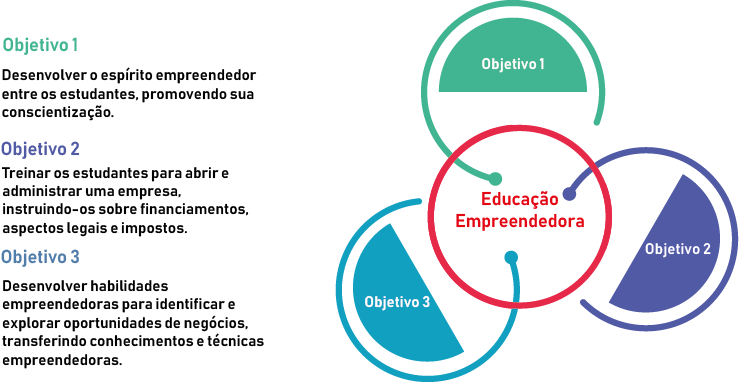
\includegraphics[scale=0.3]{Imagens/figura2.png}
\fonte{Adaptado de \cite{european_commission_best_2008}}
\label{figura_2}
\end{figure}

%\section{Inovação}
\section{Agritechs}

Independente to tamanho e demanda que venha a ter o proprietário rural, a natureza negocial do empreendimento rural e a estratégia de custo como fator de competitividade. O grande produtor para atingir este objetivo manter sua margem de lucro na entrega de seus produtos em grande escala reduzindo assim os cursos na fase da produção, já o pequeno produtor compete não em custo quantidade e sim em diferenciação dada a inferior economia de escala \cite{soares_relacao_2017}. Uma das alternativas possíveis para aumentar a lucratividade do pequeno produtor rural é o investimento em tecnologia e inovação em toda sua cadeia produtiva, tais como sementes melhoradas, adubação agrícola mais eficiente, centros coletivos de pesquisa direcionadas ao campo (Universidade-Empresa) \cite{bochi_dorneles_coletivos_2014, gomes_inovacao_2014} e Startups, estas objetivam melhoria em determinada área agropecuária \cite{junior_agtechs:_2019}. Essas empresas de base tecnológica, focadas em soluções para o agronegócio, muitas vezes são referenciadas como um setor: \textit{Agtech} \cite{blanco_agtechs:_2019}. Segundo \citeonline{junior_agtechs:_2019} as principais áreas de atuação destas Startups são as áreas de: Biotecnologia Alimentos inovadores, Marketplaces do agronegócio e restaurantes, Bioenergia e Biomateriais, Software de Gerenciamento de Fazenda, Sensores e Internet das Coisas (IoT), Robótica Agrícola, Mecanização e Equipamentos, Tecnologias da Cadeia de Suprimentos, Novos sistemas agrícolas, Varejo e Restaurante Mercearias e Conveniências digitais, Tecnologias de Casa e Cozinha e Restaurantes Online e Kits de Refeições.




\section{Inovação e Propriedade Intelectual no meio rural}

As mudanças no cenário das Propriedades Intelectuais (PI) e do desenvolvimento tecnológico levantam inúmeras questões sobre o papel que os sistemas de registro e divulgação para PI desempenham no desenvolvimento econômico do país \cite{segala_os_2016}. Em suma, os países que apresentam uma economia mais forte, dispõe de um sistema de proteção de propriedade mais robusto e confiável, em decorrência, maior quantidade de registro e depósitos das mais variadas finalidades \cite{mueller_universidades_2014}. Consequentemente os esforços dos escritórios especializados e de pesquisadores acadêmicos desses países levaram à criação de bases de micro dados sobre PI – que permite maiores possibilidades investigativas, podendo determinar preliminarmente a relevância e direcionamento das futuras produções \cite{luna_impacto_2006}. 

\clearpage
%\emph{abntex2} comando para deixar letras em itálico
%\textbf{abntex2} comando para deixar letras em negrito








